% Chapter 6: Experimental Analysis
\section{实验对比分析}

\subsection{实验方案设计}

\subsubsection{评价指标}

我们使用以下指标评估三种索引的性能:
\begin{itemize}
    \item \textbf{构建时间}:索引构建耗时(毫秒)
    \item \textbf{构建距离计算次数}:构建过程中的距离函数调用次数
    \item \textbf{树高度}:索引树的层数
    \item \textbf{节点数}:索引树的总节点数
    \item \textbf{查询距离计算次数}:查询过程中的距离函数调用次数
    \item \textbf{剪枝率}:$1 - \frac{\text{查询距离计算次数}}{\text{数据总量}}$
\end{itemize}

\subsubsection{实验变量}

\begin{itemize}
    \item \textbf{数据集类型}:低维向量、高维向量、蛋白质序列
    \item \textbf{数据规模}:500-1000
    \item \textbf{查询半径}:不同大小的查询半径
    \item \textbf{k值}:kNN查询的k值
    \item \textbf{参数配置}:叶子节点大小、pivot选择策略
\end{itemize}

\subsubsection{控制变量}

为保证实验公平性:
\begin{itemize}
    \item 三种索引使用相同的\texttt{MultiPivotSelector}选择pivot
    \item 使用相同的\texttt{TreeConfig}配置
    \item 使用相同的查询对象集合
    \item 固定随机种子(seed=42)确保可重复性
\end{itemize}

\subsection{实验环境}

实验在以下环境中进行:
\begin{itemize}
    \item 操作系统:Windows 11
    \item CPU:Intel Core
    \item 内存:16GB
    \item Java版本:Java 11
    \item 构建工具:Maven 3.8+
\end{itemize}

\subsection{索引构建性能对比}

\subsubsection{实验1:低维向量数据集(2维)}

数据集:1000个聚类分布的2D向量点。

\begin{table}[htbp]
    \centering
    \caption{实验1:低维向量数据集构建性能}
    \label{tab:exp1-build}
    \begin{tabular}{lcccc}
        \toprule
        \textbf{Index} & \textbf{Build Time (ms)} & \textbf{Dist. Comp.} & \textbf{Height} & \textbf{Nodes} \\
        \midrule
        MVP Tree & 10 & 14755 & 4 & 242 \\
        CGH Tree & 4 & 21555 & 7 & 157 \\
        LP Tree & 5 & 14755 & 4 & 242 \\
        \bottomrule
    \end{tabular}
\end{table}

\textbf{分析}:MVP树和LP树具有相同的构建距离计算次数和树结构,因为它们使用相同的划分策略(中位数划分产生8个子区域)。CGH树的距离计算次数较多,树高度更高,但节点数更少。

\subsubsection{实验2:高维向量数据集(10维)}

数据集:500个均匀分布的10D向量点。

\begin{table}[htbp]
    \centering
    \caption{实验2:高维向量数据集构建性能}
    \label{tab:exp2-build}
    \begin{tabular}{lcccc}
        \toprule
        \textbf{Index} & \textbf{Build Time (ms)} & \textbf{Dist. Comp.} & \textbf{Height} & \textbf{Nodes} \\
        \midrule
        MVP Tree & 2 & 5983 & 3 & 182 \\
        CGH Tree & 1 & 8694 & 5 & 136 \\
        LP Tree & 1 & 5983 & 3 & 182 \\
        \bottomrule
    \end{tabular}
\end{table}

\subsubsection{实验3:蛋白质序列数据集}

数据集:960条酵母蛋白质序列(长度6),使用编辑距离。

\begin{table}[htbp]
    \centering
    \caption{实验3:蛋白质序列数据集构建性能}
    \label{tab:exp3-build}
    \begin{tabular}{lcccc}
        \toprule
        \textbf{Index} & \textbf{Build Time (ms)} & \textbf{Dist. Comp.} & \textbf{Height} & \textbf{Nodes} \\
        \midrule
        MVP Tree & 14 & 12278 & 3 & 109 \\
        CGH Tree & 9 & 13662 & 4 & 57 \\
        LP Tree & 6 & 12278 & 3 & 109 \\
        \bottomrule
    \end{tabular}
\end{table}

\textbf{构建性能总结}:
\begin{itemize}
    \item MVP树和LP树的构建开销相近
    \item CGH树的构建距离计算次数较多,但树结构更紧凑
    \item 蛋白质序列数据的构建时间相对较长(编辑距离计算复杂)
\end{itemize}

\subsection{范围查询性能对比}

\subsubsection{实验1:低维向量数据集}

在不同查询半径下测试范围查询性能。

\begin{table}[htbp]
    \centering
    \caption{实验1:低维向量范围查询性能}
    \label{tab:exp1-range}
    \begin{tabular}{lccccc}
        \toprule
        \textbf{Radius} & \textbf{Linear} & \textbf{MVP} & \textbf{CGH} & \textbf{LP} & \textbf{MVP Prune\%} \\
        \midrule
        1.0 & 1000 & 119 & 367 & 218 & 88.1\% \\
        2.0 & 1000 & 168 & 596 & 371 & 83.2\% \\
        3.0 & 1000 & 201 & 985 & 594 & 79.9\% \\
        \bottomrule
    \end{tabular}
\end{table}

\begin{figure}[htbp]
    \centering
    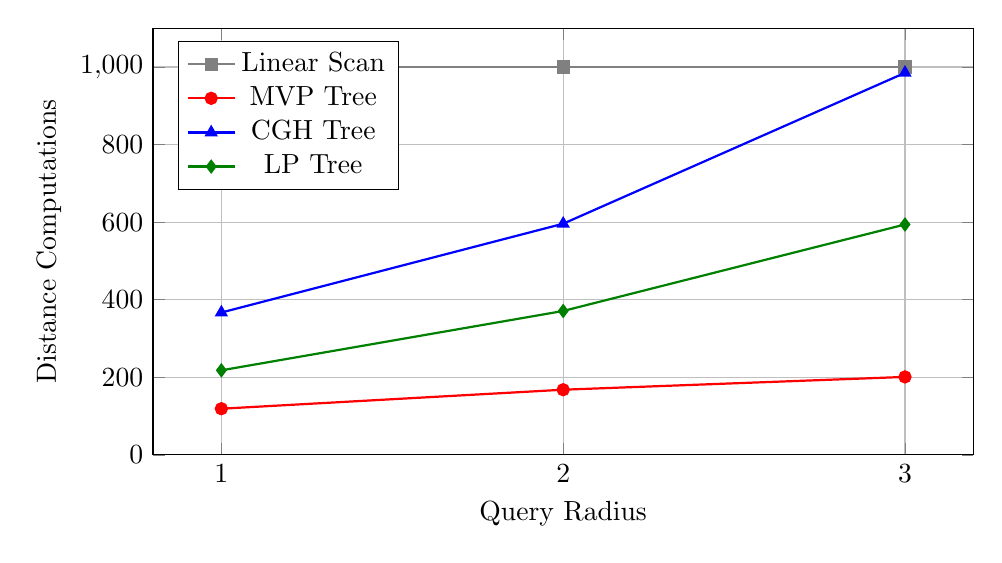
\begin{tikzpicture}
        \begin{axis}[
            width=12cm,
            height=7cm,
            xlabel={Query Radius},
            ylabel={Distance Computations},
            legend pos=north west,
            grid=major,
            xtick={1.0, 2.0, 3.0},
            ymin=0,
            ymax=1100
        ]
        \addplot[color=gray,mark=square*,thick] coordinates {(1.0,1000) (2.0,1000) (3.0,1000)};
        \addplot[color=red,mark=*,thick] coordinates {(1.0,119) (2.0,168) (3.0,201)};
        \addplot[color=blue,mark=triangle*,thick] coordinates {(1.0,367) (2.0,596) (3.0,985)};
        \addplot[color=green!50!black,mark=diamond*,thick] coordinates {(1.0,218) (2.0,371) (3.0,594)};
        \legend{Linear Scan, MVP Tree, CGH Tree, LP Tree}
        \end{axis}
    \end{tikzpicture}
    \caption{低维向量数据集范围查询距离计算次数对比}
    \label{fig:exp1-range-chart}
\end{figure}

\subsubsection{实验2:高维向量数据集}

\begin{table}[htbp]
    \centering
    \caption{实验2:高维向量范围查询性能}
    \label{tab:exp2-range}
    \begin{tabular}{lccccc}
        \toprule
        \textbf{Radius} & \textbf{Linear} & \textbf{MVP} & \textbf{CGH} & \textbf{LP} & \textbf{MVP Prune\%} \\
        \midrule
        2.0 & 500 & 73 & 140 & 73 & 85.4\% \\
        3.0 & 500 & 113 & 491 & 113 & 77.4\% \\
        4.0 & 500 & 149 & 492 & 149 & 70.2\% \\
        \bottomrule
    \end{tabular}
\end{table}

\textbf{分析}:在高维数据上,当查询半径增大时,CGH树的剪枝效果急剧下降,而MVP树和LP树仍保持较好的剪枝率。

\subsubsection{实验3:蛋白质序列数据集}

\begin{table}[htbp]
    \centering
    \caption{实验3:蛋白质序列范围查询性能}
    \label{tab:exp3-range}
    \begin{tabular}{lcccc}
        \toprule
        \textbf{Radius} & \textbf{Linear} & \textbf{MVP} & \textbf{CGH} & \textbf{LP} \\
        \midrule
        1.0 & 960 & 233 & 515 & 233 \\
        2.0 & 960 & 767 & 515 & 767 \\
        3.0 & 960 & 771 & 960 & 771 \\
        \bottomrule
    \end{tabular}
\end{table}

\textbf{分析}:蛋白质序列数据的编辑距离值域较小(0-6),导致查询半径对剪枝效果影响显著。半径为1时剪枝效果好,半径增大后剪枝效果快速下降。

\subsection{kNN查询性能对比}

\subsubsection{低维向量数据集kNN查询}

\begin{table}[htbp]
    \centering
    \caption{低维向量kNN查询性能}
    \label{tab:exp1-knn}
    \begin{tabular}{lccccc}
        \toprule
        \textbf{k} & \textbf{Linear} & \textbf{MVP} & \textbf{CGH} & \textbf{LP} & \textbf{MVP Prune\%} \\
        \midrule
        5 & 1000 & 37 & 457 & 37 & 96.3\% \\
        10 & 1000 & 51 & 538 & 51 & 94.9\% \\
        20 & 1000 & 77 & 558 & 77 & 92.3\% \\
        \bottomrule
    \end{tabular}
\end{table}

\textbf{分析}:MVP树和LP树在kNN查询上表现优异,剪枝率超过90\%。CGH树的kNN查询效果相对较差。

\subsubsection{高维向量数据集kNN查询}

\begin{table}[htbp]
    \centering
    \caption{高维向量kNN查询性能}
    \label{tab:exp2-knn}
    \begin{tabular}{lccccc}
        \toprule
        \textbf{k} & \textbf{Linear} & \textbf{MVP} & \textbf{CGH} & \textbf{LP} & \textbf{MVP Prune\%} \\
        \midrule
        5 & 500 & 433 & 500 & 433 & 13.4\% \\
        10 & 500 & 480 & 500 & 480 & 4.0\% \\
        20 & 500 & 482 & 500 & 482 & 3.6\% \\
        \bottomrule
    \end{tabular}
\end{table}

\textbf{分析}:高维数据受维度灾难影响严重,所有索引的kNN查询剪枝效果都大幅下降,接近线性扫描。

\subsection{参数影响分析}

\subsubsection{最大叶子节点大小的影响}

使用300个数据点测试不同叶子节点大小对性能的影响。

\begin{table}[htbp]
    \centering
    \caption{叶子节点大小对树结构和查询性能的影响}
    \label{tab:leaf-size-impact}
    \begin{tabular}{ccccccc}
        \toprule
        \textbf{Leaf Size} & \textbf{MVP H} & \textbf{CGH H} & \textbf{LP H} & \textbf{MVP Dist} & \textbf{CGH Dist} \\
        \midrule
        5 & 4 & 7 & 4 & 87 & 299 \\
        10 & 4 & 6 & 4 & 112 & 299 \\
        25 & 3 & 6 & 3 & 141 & 299 \\
        50 & 2 & 4 & 2 & 214 & 299 \\
        100 & 2 & 2 & 2 & 214 & 299 \\
        \bottomrule
    \end{tabular}
\end{table}

\textbf{分析}:叶子节点大小影响树高度。较小的叶子节点产生更深的树,可能有更好的剪枝效果,但也增加了节点访问开销。

\subsubsection{Pivot选择策略的影响}

\begin{table}[htbp]
    \centering
    \caption{Pivot选择策略对性能的影响}
    \label{tab:pivot-strategy-impact}
    \begin{tabular}{lcccc}
        \toprule
        \textbf{Strategy} & \textbf{MVP Build} & \textbf{CGH Build} & \textbf{MVP Query} & \textbf{CGH Query} \\
        \midrule
        RANDOM & 3810 & 5895 & 200 & 300 \\
        FFT & 6150 & 8702 & 141 & 299 \\
        MAX\_SPREAD & 25679 & 42909 & 168 & 500 \\
        \bottomrule
    \end{tabular}
\end{table}

\textbf{分析}:
\begin{itemize}
    \item RANDOM策略构建开销最小,但查询性能一般
    \item FFT策略在构建开销和查询性能之间取得较好平衡
    \item MAX\_SPREAD策略构建开销最大,查询性能不稳定
\end{itemize}

\subsection{结果分析与讨论}

\subsubsection{三种索引性能总结}

\begin{table}[htbp]
    \centering
    \caption{三种索引性能总结}
    \label{tab:performance-summary}
    \begin{tabular}{lccc}
        \toprule
        \textbf{Aspect} & \textbf{MVP Tree} & \textbf{CGH Tree} & \textbf{LP Tree} \\
        \midrule
        Build Efficiency & Medium & Higher Overhead & Medium \\
        Tree Balance & Good & Variable & Good \\
        Range Query (Low-dim) & Excellent & Good & Good \\
        Range Query (High-dim) & Good & Poor & Good \\
        kNN Query & Excellent & Poor & Excellent \\
        Large Radius Query & Good & Poor & Good \\
        \bottomrule
    \end{tabular}
\end{table}

\subsubsection{性能差异原因分析}

\textbf{MVP树和LP树}:
\begin{itemize}
    \item 使用相同的划分策略(中位数划分产生8个子区域)
    \item 剪枝条件相同,因此查询性能非常接近
    \item 具有包含规则,可以批量返回结果
\end{itemize}

\textbf{CGH树}:
\begin{itemize}
    \item 只有4个子区域,划分粒度较粗
    \item 基于距离差符号划分,平衡性依赖数据分布
    \item 剪枝条件需要$|d_1 - d_2| > 2r$才能生效,大半径时失效
    \item 没有包含规则
\end{itemize}

\subsubsection{适用场景建议}

基于实验结果,我们给出以下建议:

\begin{itemize}
    \item \textbf{低维聚类数据}:推荐使用MVP树或LP树
    \item \textbf{高维数据}:三种索引效果都一般,但MVP树和LP树相对更好
    \item \textbf{小查询半径}:三种索引效果都好
    \item \textbf{大查询半径}:避免使用CGH树
    \item \textbf{kNN查询}:推荐使用MVP树或LP树
    \item \textbf{序列数据}:根据编辑距离值域选择合适的查询半径
\end{itemize}
